\BourbakiUnnumberedChapter{表格}{表格}

约定（参见 IV 第 66 页）。

形如 \(p^{\alpha} \cdot q^{\beta} \ldots\) 的记号，其中 \(p, q, \alpha, \beta, \ldots\) 是整数 \(\geqslant 1\)，表示 \(D_{k}\)（其中 \(k = p\alpha + q\beta + \cdots\)）的一个元素，它有 \(\alpha\) 个分量等于 \(p, \beta\) 个分量等于 q，等等。于是 \(3 \cdot 1^{2}\) 表示 \(D_{5}\) 中等于 (3, 1, 1, 0, 0) 的元素，而 \(1^{4}\) 表示 \(D_{4}\) 的元素 (1, 1, 1, 1)。

在指标为 \(\alpha\) 的行（属于矩阵 \(C\)）的右侧，给出了 \(S(\alpha)\) 作为 \(s_1, \ldots, s_k\) 中单项式的表达式。例如，对 \(k = 3\) 与 \(\alpha = 2.1\)，我们有

\[
\mathrm{S} (2. 1) = s _ {1} s _ {2} = \mathrm{M} (2. 1) + 3 \mathrm{M} \left(1 ^ {3}\right).
\]

我们对矩阵 D 的列采用了相应的约定。例如，对 \(k = 4\) 与 \(\alpha = 2^2\)，我们有

\[
\mathbf {M} (2 ^ {2}) = 2 s _ {4} - 2 s _ {1} s _ {3} + s _ {2} ^ {2}.
\]

我们回顾， \(\mathbf{M}(2^2)\) 是所有形如 \(\mathbf{X}_i^2\mathbf{X}_j^2\)（对 \(1 \leqslant i < j \leqslant n\)）的单项式在环 \(\mathbf{Z}[\mathbf{X}_1, \ldots, \mathbf{X}_n]\) 中的和。

空框表示矩阵 C 和 D 的零元素。

矩阵 D\\
\(k = 2\)\\
\pandocbounded{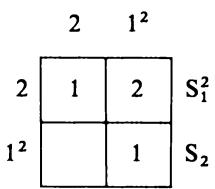
\includegraphics[keepaspectratio]{images/part001_666ab4c0.jpg}}

\pandocbounded{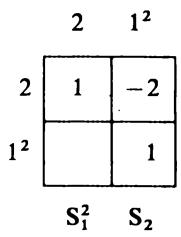
\includegraphics[keepaspectratio]{images/part001_442e375f.jpg}}

\(k = 3\)

3

2.1

\(1^{3}\)

3

1

3

6

\(S_{1}^{3}\)

2.1

1

3

\(S_{1}S_{2}\)

\(1^{3}\)

1

\(S_{3}\)

3 2.1 \(1^{3}\)\\
\pandocbounded{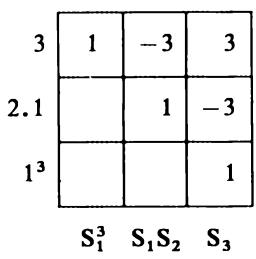
\includegraphics[keepaspectratio]{images/part001_fb1fe29f.jpg}}

\(k = 4\)

4

1

4

6

12

24

\(S_{1}^{4}\)

3.1

1

2

5

12

\(S_{1}^{2}S_{2}\)

\(2^{2}\)

1

2

6

\(S_{2}^{2}\)

\(2.1^{2}\)

1

4

\(S_{1}S_{3}\)

\(1^{4}\)

1

\(S_{4}\)

矩阵C

\pandocbounded{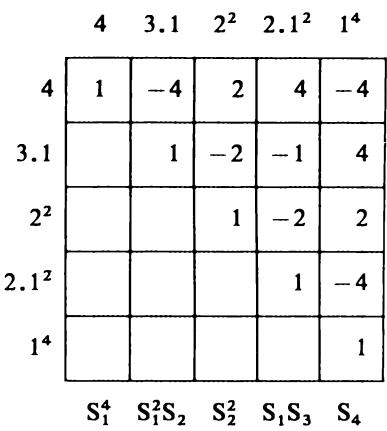
\includegraphics[keepaspectratio]{images/part001_bf35a948.jpg}}

\pandocbounded{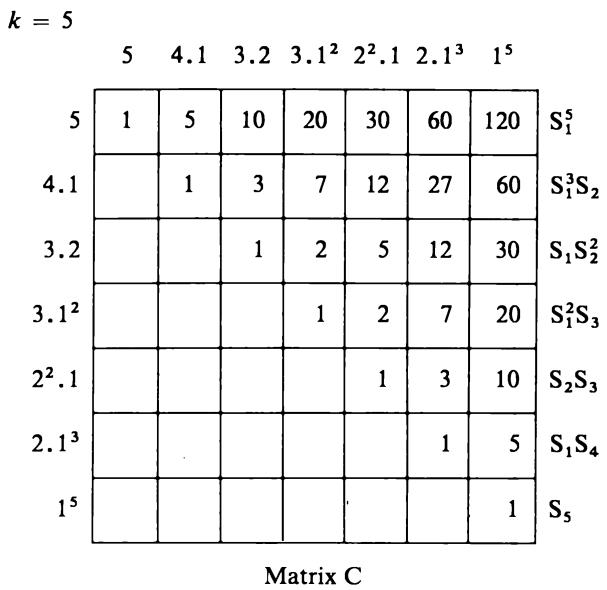
\includegraphics[keepaspectratio]{images/part001_7e862639.jpg}}

\pandocbounded{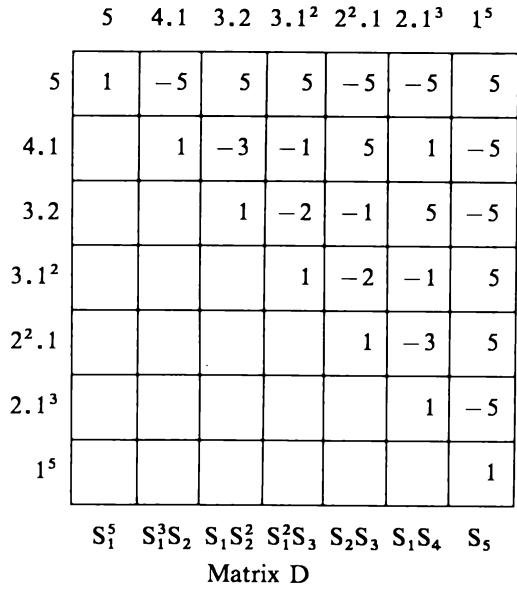
\includegraphics[keepaspectratio]{images/part001_eab66d56.jpg}}


